\documentclass[12pt,a4paper]{amsart}
\usepackage[utf8]{inputenc}
\usepackage{amsmath}
\usepackage{amsfonts}
\usepackage{amssymb}

\usepackage{hyperref}

\usepackage{float}
\usepackage{subfig}


%\usepackage[dvipdfmx]{graphicx}
\usepackage{graphicx}
\usepackage{caption}
%\usepackage[nobysame, alphabetic]{amsrefs}
%\usepackage{here}
%\usepackage{showkeys}
\newcommand{\modif}{$\clubsuit$}
\newtheorem{thm}{Theorem}[section]
\newtheorem{defn}[thm]{Definition}
\newtheorem{coro}[thm]{Corollary}
\newtheorem{prop}[thm]{Proposition}
\newtheorem{lem}[thm]{Lemma}
%\theoremstyle{definition}
\newtheorem{rmk}[thm]{Remark}
\newtheorem{cond}[thm]{Condition}

%CB defs
\def\rh{\phi_h}
\def\rv{\phi_v}

\def\HH{\mathbb{H}}
\def\dHH{\partial \mathbb{H}}
\def\hd{\hat{\delta}}
\def\ha{\hat{\alpha}}
\def\haa{\ha \cup \{\alpha^+,\alpha^-\}}

\def\im{\mathrm{Im}\,}
\def\re{\mathrm{Re}\,}
\def\oo{\HH / \Gamma_0(2)} 
\def\g2{\Gamma(2)}
\def\go2{\Gamma_0(2)}
\def\ah{\Gamma_0^t(2)}
\def\oot{\HH / \ah} 
\def\xx{\HH/\g2}


\def\ZZ{\mathbb{Z}}
\def\CC{\mathbb{C}}
\def\RR{\mathbb{R}}
\def\QQ{\mathbb{Q}}
\def\NN{\mathbb{N}}

\def\tt{\Sigma_{1,1}}

\def\fp{\mathbb{F}_p}
\def\aut{\text{Aut}(\F2)}
\def\gl2{\mathrm{GL}(2, \ZZ)}
\def\sl2{\mathrm{SL}(2, \ZZ)}
\def\slc{\mathrm{SL}(2, \CC)}

\def\oi{\Gamma.\{i\}}

\def\gg{\mathcal{G}_n}
\def\ggp{\mathcal{G}_p}

\def\isom{\mathrm{isom}(\HH)}

\def\isomH{\text{isom}^+(\HH)}
\def\tr{\text{tr\,}}


\def\GI{\mathbb{Z}[i]}
\def\hc{\CC \setminus \GI}



\title{Geodesics and values of quadratic forms}

 \author[McShane]{Greg McShane}
 % \author[Vlad]{Vlad Sergesciu}
\address{Institut Fourier 100 rue des maths, BP 74, 38402 St Martin d'H\`eres cedex, France}
\email{mcshane at univ-grenoble-alpes.fr}




\begin{document}

\maketitle

\section{Introduction}

	

\begin{thm}\label{triv}
Let $p$ be a prime then the equation
$$x^2 = -1$$
admits a solution in $\fp$ iff 
$p =2$ or $p-1$ is a multiple of $4$.
\end{thm}


\begin{thm}[Fermat]\label{main}
Let $p$ be a prime then the equation
$$x^2 + y^2 = p $$
has a solution in integers  iff  $p =2$ or $p-1$ is a multiple of $4$.
\end{thm}

There are many proofs of these theorems but the approach initiated
by Heath-Brown in \cite{heath} has inspired many admirers if not 
imitators see for example the very nice account of Elsholtz \cite{elsholtz}.
In some senses this manuscript is a companion 
to Elsholtz's where instead of looking at the number theory as combinatorics we work in an explicitly geometric context.
As such we refer the reader to Elsholtz for historical perspective
and the like.

\subsection{Involutions}

The essential ingredients in the Heath-Brown paper are:
a finite set $X$ equipped with a pair of involutions such that:


\begin{itemize}
	\item Any fixed point of the one of the involutions,
		should it exist, is a solution of the equation;
	\item The other involution has a unique fixed point which is easy to compute.
\end{itemize}

The existence of the unique fixed point of the second involution
allows one to conclude that  the $X$ has an odd number of elements
and so that any involution has a fixed point.

Probably the most elegant incarnation of this method is Dolan's
proof \cite{dolan}.

\subsection{Arcs on a punctured surface}

The starting point for this work was a series of observations
concerning $\lambda$-lengths of simple arcs on a once punctured
torus equipped with a hyperbolic structure for example $\HH/\Gamma'$
where $\Gamma' < \sl2$ is the commutator subgroup. 
The reader, unfamiliar with the relationship between hyperbolic
geometry and number theory,
should consult Springborn's articles \cite{springborn1, springborn2}
where a dictionary between geometric and number theoretic notions is presented.

An important
feature of a punctured surface is that it admits \textit{uniform
cusp regions} that is there is a neighborhood of each puncture, or more properly cusp, isometric to 
$$\{z\in \mathbb{H}, \mathrm{Re}z \geq 1\}/\langle z \mapsto z+2 \rangle$$  
The  torus $\mathbb{H}/\Gamma'$ can
be obtained from a pair of ideal triangles by "gluing" and the sides
of the ideal triangles form a triple of complete simple geodesics on
the surface. The corners of the triangles glue up to a neighborhood
of the puncture. We define an \textit{arc} to
be any complete geodesic on a punctured surface with both of its
ends terminating at cusps. The three sides of the ideal triangle(s)
above form a triple of disjoint simple arcs. Each of these arcs has
infinite length but if we only consider the portion outside the
uniform cusp region then its length is finite. The $\lambda$-length
of the arc is exponential of half the length of this finite portion.
Whilst this definition works well for simple arcs, since the portion of
the arc
outside the uniform cusp region is connected, more care is needed if
the arc is not simple.

Since Penner first defined $\lambda$-length 
there has been much work on their applications

\begin{itemize}
	\item Weil-Peterson volume of moduli space \cite{bob}
	\item cluster algebras \cite{Fomin}.
	\item Conway-Coxeter frieze patterns \cite{frieze}.
\end{itemize}
Our approach depends on determining the number of arcs on a surface
of $\lambda$-length p.
Probably the easiest surface to count arcs on is $\xx$.

\begin{thm}\label{g2 arcs}
	Let $p$ be a prime number then the number of arcs of
	$\lambda$-length p on the surface
	$\xx$ is $3(p-1)$.
\end{thm}


 \begin{figure}[H]
\begin{center}
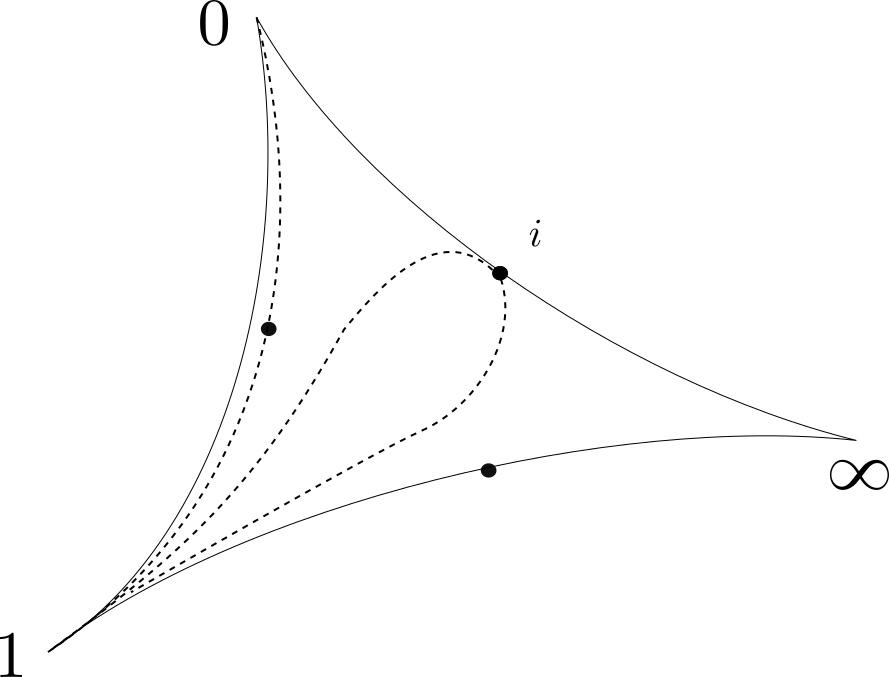
\includegraphics[scale=.3]{3sphere.png} 
\end{center}
\caption{The surface $\xx$. The dotted lines are arcs one of which
is a loop of $\lambda$-length 2, and the other has $\lambda$-length 1.}
\label{3sphere}
\end{figure}

The surface is $\xx$ is not compact and has three cusps which, as we
shall see, are naturally associated with $0,1,\infty \in \partial \mathbb{H}$.
This is a manifestation of the fact that $\g2$ acts on the extended
rationals $\mathbb{Q} \cup \{\infty\}$.
By \textit{parity} we mean one
of the three classes one obtains by taking the 
numerator and denominator of $\frac{p}{q}$ modulo 2
where, by convention, $\infty = \frac{1}{0}$.
Actually $\xx$ is a degree 6 cover of the modular surface
$\mathbb{H}/\Gamma$. 
Unfortunately this covering is ramified at 2 points and
the projection of an arc on $\xx$ may or may not be an arc.
The problem lies in that an arc may be invariant by some involution
in the covering group and as a consequence connects the cusp on
$\mathbb{H}/\Gamma$ to a ramification point.
In fact 


\begin{thm}\label{modular arcs}
	Let $p$ be a prime number then the number of arcs of
	$\lambda$-length p on the modular surface
	$\mathbb{H}/\Gamma$ is 
	
	\begin{itemize}
		\item p-1 if 4 does not divide p-1,
		\item p-2 if p=2 or 4 divides p-1.
	\end{itemize}

	% \begin{itemize}
	% 	\item p-1 if p-1 and  12 are coprime
	% 	\item p-3 if p is of the form $12k +1$
	% 	\item p-2 if p is of the form $12k+7$, $12k
	% 		+5$ or $12k + 9$
	% \end{itemize}

\end{thm}

As we shall see in Section \ref{}, this result is indeed equivalent to Theorem \ref{main}. 

Computing the $\lamda$-length of an arc $\alpha$ on $\xx$ 
is relatively simple.
One considers a lift $\hat{\alpha}$ of the arc.
This is a Poincaré geodesic joining a pair of distinct rationals
$a/c,b/d \in \mathbb{Q}$ and the $\lambda$-length is just
the determinant of the matrix
$$ 
 \begin{pmatrix} a & b \\ c & d \end{pmatrix}.
$$
Evidently the arcs on $\xx$ fall into two families:
\begin{itemize}
	\item arcs that join distinct cusps. 
	\item arcs that have both ends at the same cusp
\end{itemize}
We will refer to the second kind of arc as a \textit{loops}
(see Figure \ref{3sphere}).
Amusingly one can characterise loops using $\lambda$-lengthis.
\begin{lem}
	An arc on $\xx$ is a loop if and only if its
	$\lambda$-length is even.
\end{lem}


\section{Klein four group and the Burnside Lemma}

We give a proof of Theorem \ref{triv} using the Burnside Lemma.


Recall that if $G$ is  a group acting on a finite set $X$ then the Burnside Lemma says
\begin{equation}\label{burnside}
|G| |X/G| = \sum_{g} |X^g| 
\end{equation}  
where, as usual, 
 $X^g$ denotes the set of fixed points of the element $g$ 
 and $X/G$  the orbit space.

Let $p\neq 2$,  $X = \fp^*$ and $G$ be the group generated by the two involutions
\begin{eqnarray*}
x & \mapsto -x \\
x & \mapsto 1/x.
\end{eqnarray*}
The group  $G$ has exactly four elements namely:
\begin{itemize}
\item the trivial element which has  $p-1$ fixed points
\item $x\mapsto -x$ which has no fixed points 
\item  $x\mapsto 1/x$ has exactly two fixed points namely $1$ and $-1$.
\item  $g:x \mapsto -1/x$ is the remaining element and the theorem is equivalent to the existence of a fixed point for it.
\end{itemize}
Note that since $\fp$ is a field 
$|X^g| = \sharp \{x^2 = -1, \, x\in \fp^* \}$
is either $0$ or $2$.
Now for our choice of $X$ and $G$ equation (\ref{burnside}) yields
\begin{equation}
4 |X/G|   = (p-1) + 2 + |X^g|.
\end{equation}  
The LHS is always divisible by $4$ so the  RHS is too and
it follows from this that
$$ |X^g|. = \left\{  \begin{array}{ll}
		0 & \text{if }(p-1) =  2 \mod 4 \\
2 & \text{if }(p-1) =  0 \mod 4 \\
\end{array}
\right.
$$
This proves Theorem \ref{triv}.

\subsection{Extending}

Thus we have shown that $-1$ is a quadratic residue modulo $p$ if
$p$ is of the form $4k+1$. 
It is natural to consider the other questions considered by Fermat:
namely for which values of $p$ are $-2$ and $-3$ residues?

In fact  $-2$  is a residue if $p$ is $2$ or of the form $8k+1$ or $8k+3$.
Showing this in the spirit of Heath-Brown requires one to consider a group generated by the involutions 
\begin{eqnarray*}
x & \mapsto -x \\
x & \mapsto 2/x.
\end{eqnarray*}
One immediately sees that things are more complicated as the
second involution has fixed points if and only if $2$ is a residue
whereas $x\mapsto 1/x$ always had exactly two fixed points.
Thus there are two cases:
\begin{itemize}
	\item $p=8k+1$ and both $2$ and $-2$ are residues
	\item $p=8k+3$ and $-2$ is a residue but $2$ is not.
\end{itemize}
To prove this second assertion 
one must show that 
$x  \mapsto 2/x$ has no fixed point
% so $2$ is not a residue 
so that, by Burnside,
$x  \mapsto -2/x$ has two fixed points 
both of which are square roots of $-2$.
Thus one must show that the only solution of the associated diophantine equation 
$$np = x^2 - 2y^2,$$
is the trivial solution $n=x=y=0$.
Now using the fact that 
$x^2 - 2y^2$ 
is the norm of $x+y \sqrt{2}\in \mathbb{Z}[\sqrt{2}]$ which is a
euclidean ring for this norm,
one reduces to considering just the solutions of 
$$p = x^2 - 2y^2.$$
Finally, 
% by considering congruence classes modulo 8,
one concludes by showing that if $x,y$ are integers then
$x^2 - 2y^2$ never takes the value $3 \mod 8$.

\subsection{The case $p=11$}

The first real case of interest in understanding 
$x\mapsto -2/x$ is that of $\mathbb{F}_{11}^*$.
Evidently, $11 = 3^2 + 2\times 1^2$ so that 
$\bar{3}$ and $-\bar{3} = \bar{8}$ rare the fixed points of the involution.


The reduction homomorphism $x\mapsto \bar{x}$
allows one to identify the elements of $\fp$
with the equivalence classes that constitute
 the quotient $\mathbb{Z}/p \mathbb{Z} $.
It is the usual  
to choose the integers $0,1, 2\ldots p-1&$ as representatives for the
latter, 
however, we shall find it convenient to work with
another set of representatives, the even integers 
$0, 2, 4 \ldots 2p -2$.
Using the euclidean algorithm to compute $\bar{x}^{-1} \in \mathbb{F}_{11}$
we have the following table:
\vspace{.1in}
\begin{center}
	
\begin{tabular}{|c|c|c|c|c|c|c|c|c|c|c|}
	\hline
	${x}$ & 12 & 2 & 14 & 4 & 16 & 6 & 18 & 8 & 20 & 10 \\
	\hline
	$\bar{x}$ & 1 & 2 & 3 & 4 & 5 & 6 & 7 & 8 & 9 & 10 \\

	\hline
	$\bar{x}^{-1}$& 12 & 6 & 4 & 14 & 20 & 2 & 8 & 18 & 16 & 10 \\
	\hline
$-2\bar{x}^{-1}$& 20 & 10 & 14 & 16 & 4 & 18 & 6 & 8 & 12 & 2 \\
	\hline
\end{tabular}
\end{center}
\vspace{.1in}
One notes that there are two fixed points of $-\bar{x} \mapsto
-2\bar{x}^{-1}$ namely $\overline{14}=\bar{3}$ and $\bar{8}$.


\section{Counting sums of squares}

We count solutions for the diophantine problem $n = mc^2 + d^2$ in
two ways:
\begin{itemize}
	\item Firstly by showing that solutions are
		naturally associated to the  $\Gamma$
		orbit of $i\sqrt m$;
	\item Secondly by counting arcs of $\lambda$-length n.
\end{itemize}


\subsection{From solutions to $\Gamma$ orbits}

The transformation $z \mapsto z + 1$ generates an infinite cyclic
group acting on $\mathbb{H}$.
The standard fundamental domain for this group is an infinite strip,
which we will refer to as the \textit{fundamental strip},
consisting of all the $z\in \CC$ such that 
the real part is between $0$ and $1$.

\begin{lem} \label{squares}
Let $n\geq2$ be an integer.
The number of  ways of writing $n$  as a  sum of squares
$$n = c^2 + d^2$$
with $c,d$ coprime integers
is equal to the number of points
of $\oi$, 
the $\sl2$  orbit of $i$,
in the fundamental strip such that the imaginary part (euclidean height) is $\frac{1}{n}$.
\end{lem}
Note that we are counting $c^2 + d^2$ and $d^2 + c^2$ 
as \textit{different} representations of $n$.

\proof  Suppose there is a point $w$
verifying the hypotheses, in particular

$$w = \frac{ai + b}{ci + d},\, 
\text{ for some } \begin{pmatrix} a&b\\c&d
\end{pmatrix} \in \Gamma.$$
Then one has:

$$\im w = \im  \left (\frac{ai +b}{ci+d } \right)
= \frac{\im i} {c^2 + d^2},$$

so $n = c^2 + d^2$ as claimed.

Conversely if $c,d$ are coprime integers
such that $n=c^2 +d^2$
 then there exists $a,b$ such that
 $$ad - bc = 1 \Rightarrow  
A =  \begin{pmatrix}
 a & b \\
 c & d
 \end{pmatrix} \in \Gamma.
$$
%The real part of $w = \frac{ai +b}{ci+d }$ is
%$$ac + bd = (a,b).(c,d),$$
%and
By applying a suitable iterate of the parabolic transformation 
$z \mapsto z + 1$, if necessary 
one can choose $w$ such that $0 \leq \text{Re\,} w < 1$.

\hfill $\Box$

By exactly the same argument one has a slightly more general result:

\begin{lem} \label{quadratic form}
Let $n\geq2$ be an integer and $m < n$ a square free integer.
The number of  ways of writing $n$  as a  sum of squares
$$n = mc^2 + d^2$$
with $c,d$ coprime integers
is equal to the number of points
of $\Gamma.\{i\sqrt m\}  $
the $\sl2$  orbit of $i\sqrt m$,
in the fundamental strip at euclidean height $\frac{\sqrt m}{n}$.
\end{lem}


\subsection{From $\Gamma$ orbits to arcs}

Suppose that $n$ is can be written as a sum of squares $c^2 +d^2$
and $w$ is the corresponding point in the fundamental strip then we
can associate a Poincaré geodesic to $w$ in a natural way, 
we simply take the vertical line that passes through $w$.
This geodesic joins two points in the ideal boundary of $\mathbb{H}$
namely $\infty$ and $\frac{ac + bd}{n}\in \mathbb{Q}$.
Penner's $\lambda$-length
This geodesic projects to an arc on the surface $\xx$
and, using the definition above, its $\lambda$-length is $n$.
If $n$ is not even then this arc is not a loop
and so joins a pair of distinct cusps $\infty$ to $1$ say.



\section{Inversions}

We denote by $\mathbb{H}$ the Poincaré upper half plane and $\dHH$
its ideal boundary ie $\mathbb{R}\cup \{\infty\}$.
Recall that an \textit{inversion} is an orientation reversing
isometry of $\mathbb{H}\cup \dHH$. 
A Poincaré geodesic is either a vertical line or a semicircle
orthogonal to $\mathbb{R}$.
In both cases it is uniquely determined by its endpoints in the
ideal boundary.
To each Poincaré geodesic is associated a unique inversion which fixes it pointwise. 
The inversion
$\rh: z\mapsto -\bar{z}$ fixes $0$ and $\infty$ 
and so the geodesic joining them.
The group of isometries acts transitively on pairs of distinct
points $a,b \in \partial \mathbb{H}$ and so
there is an inversion that fixes the geodesic joining $a,b$which is
in fact conjugate to $\rh$.
The inversion fixing $1,-1$ is easily seen to be
$\rv:z\mapsto \frac{1}{\bar{z}}$. 

Note that if $a,b$ are coprime integers then:
\begin{itemize}
	\item
The image of $\frac{a}{b}$ under $\rh$ is $-\frac{a}{b}$
and the $\lambda$-length of the geodesic joining them is $2ab$.

	\item
The image of $\frac{a}{b}$ under $\rv$ is $\frac{b}{a}$
and the $\lambda$-length of the geodesic joining them 
is $|a^2 - b^2|$.

\end{itemize}
It follows from these remarks that:
\begin{lem}
	Let $p>2$ be a prime then:
	
\begin{itemize} 

	\item There is no arc of $\lambda$-length $p$
		invariant under $\rh$.
	\item There are exactly two arcs of $\lambda$-length
		$p$ invariant under $\rv$;

\end{itemize}
\end{lem}
\proof 
The first part is easy because the $\lambda$-length of such an arc
is an even integer.
The second part follows from the fact that p factorises as
$$p = |(a-b)| |(a+b)|,$$
so up to permutation and change of sign $a,b$ are the integers
$\frac{1}{2}(p\pm1)$.

\hfill $\Box$

\section{Congruence subgroups}

The Hecke congruence subgroup $\Gamma_0(N)$ of level $N$ is the subgroup of
$\Gamma = \mathrm{SL}(2,\ZZ)$ is a normal.
It is a subgroup of $\Gamma_0(N)$:
$$ \begin{pmatrix} a & b \\ c & d \end{pmatrix} = 
\begin{pmatrix} 1 & * \\ 0 & 1 \end{pmatrix} \mod N.$$

For $N=2$ this is generated by just two elements namely:
$$ P = \begin{pmatrix} 1 & 1 \\ 0 & 1 \end{pmatrix} \text{ and } Q=  \begin{pmatrix} 1 & 0 \\ 2 & 1 \end{pmatrix}.$$
The product $P^{-1}Q$ is an element of order $2$:
$$ P^{-1}Q = \begin{pmatrix} -1 & -1 \\ 2 & 1 \end{pmatrix}.$$
So the quotient $\oo$ is a non-compact orbifold with two cusps and a single cone point.
This orbifold admits a Klein four group as its group of orentations
and the quotient by this group is a hyperbolic triangle with angles
$0, \pi/2, \pi/4$.

 \begin{figure}[H]
\begin{center}
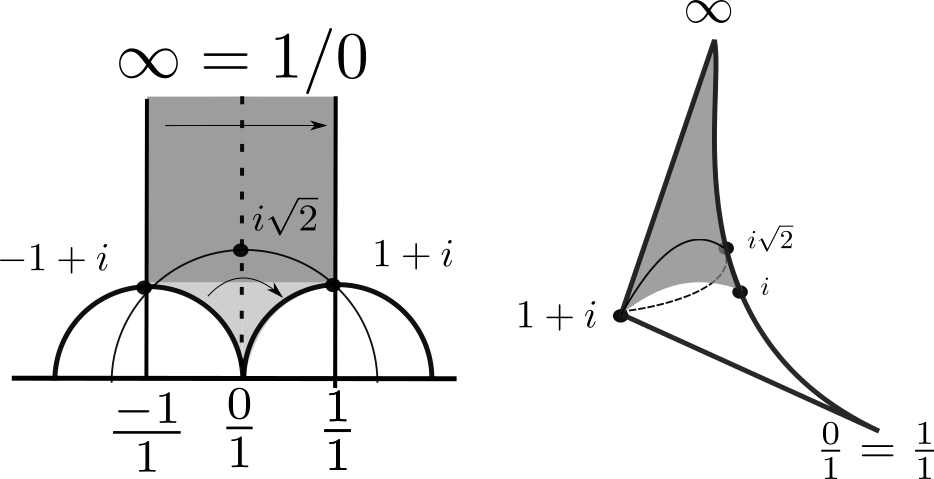
\includegraphics[scale=.5]{hecke_fund_dom.png} 
\end{center}
\caption{On the left a fundamental domain for $\ah$ with side
pairings.  On the right the quotient surface $\oot$, the dark region
is a cusp region.}
\label{fundamental domain}
\end{figure}

The action of this group on $\mathbb{Q}\cup \{\infty\}$ is not
transitive and there are two orbits.
Now $\Gamma_0(2) < \Gamma(2)$ so each of these orbits is a union of
$\Gamma(2)$-orbits.
Since $\Gamma(2)$ preserves the parity of the numerator and
denominator of a fraction there are exactly three $\Gamma(2)$ orbits
corresponding to $\frac{0}{1} = 0,\, \frac{1}{1} = 1, \,
\frac{1}{0}=\infty$.
Now since $P$ maps $0$ to one:
$$\Gamma_0(2) \{0\} =   \Gamma(2) \{0\} \cup \Gamma(2) \{1\}.$$


In the previous section we considered the action of the involution
$x\mapsto -2/x$ on $\mathbb{F}_{p}^*$. It is natural to study the
action of the corresponding involution of $\mathbb{H}$ that is
$z\mapsto -2/z$ but unfortunately this does not normalise
$\Gamma_0(2)$. 
However it does normalise the \textit{anti Hecke congruencegroup}:
$$ \ah := \left \{ \begin{pmatrix} a & b \\ c & d \end{pmatrix} = 
\begin{pmatrix} 1 & 0 \\ * & 1 \end{pmatrix} \mod N \right \} < \g2.$$
The Hecke congruence group and the anti Hecke group are isomorphic
and in fact $z\mapsto -1/z$ conjugates them  in $\Gamma$  .
We can determine the orbits of this group on $\QQ$ using this
conjugation and we have:
$$\ah \{\infty\} =   \Gamma(2) \{\infty\} \cup \Gamma(2) \{1\}.$$


We denote by $F$ the set  $\{ z, \im z > 1\}$
this is a \textit{horoball in $\HH$} centered at $\infty$.
The image of $F$ under the $\sl2$ action consists of
$F$ and infinitely many disjoint circles, the so-called \textit{Ford circles}, 
each tangent to the real line at some rational $m/n$.
We adopt the convention that $F$ is also a Ford circle of infinite radius.
If $G < \sl2$ is any finite index subgroup then 
each Ford circle projects to a cusp region on $\mathbb{H}/G$ and we
call this system  the \textit{canonical system of cusp regions}.

\begin{figure}[H]
\begin{center}
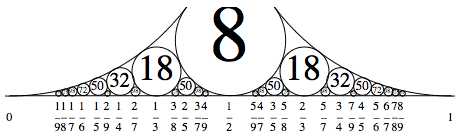
\includegraphics[scale=.8]{Ford-circles.png} 
\end{center}
\caption{Ford circles with tangent points and curvatures.
Recall that the curvature of a euclidean circle is the reciprocal of its radius.}
\end{figure}

The following is well known and is easily checked:

\begin{lem}\label{ford}
The Ford circle tangent to the real line at $m/n$
has Euclidean diameter $1/n^2$.
\end{lem}

\begin{coro}
	The $\lambda$-length of the arc joining 
	$a/c, b/d \in \mathbb{Q}$ is the absolute value of
	the determinant of the associated matrix 
	$$A= \begin{pmatrix} a& b\\c&d \end{pmatrix}.$$
\end{coro}

\proof There exists  $b'\in \mathbb{Z}$ and  a matrix $A' \in \sl2$ such that the product $A'A$
is an upper triangular matrix:
	$$A'A= \begin{pmatrix} 1& b'\\0& \det A
	\end{pmatrix}.$$
The image of $a/c$ under the Mobius transformation associated to
$A'$ is infinity and the image of $b/d$ is $b'/\det A$.
The Ford circle at $\infty$ is $F$ and the 
diameter of the circle tangent at $b'/\det A$ is $(\det A)^2$.

\hfill $\Box$

  \begin{figure}[H]
	  \label{cusp regions}
\begin{center}
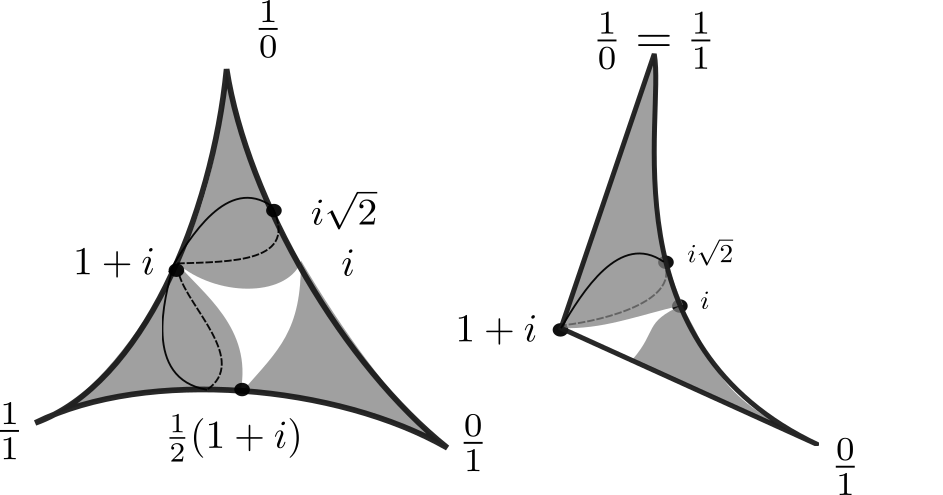
\includegraphics[scale=.5]{hecke_cover.png} 
\end{center}
\caption{On the left $\xx$ with the cusp regions inherited from the
Ford circles  $\mathbb{H}$.
On the right $\oot$ with the unmodified cusp regions.}
\end{figure}
\subsection{Cusp regions  on $\oot$}

The canonical system on $\xx$ consists of three cusp regions 
one for each of the three cusps $0,1,\infty$.
The map $z\mapsto z/z+1$ fixes $0$ and normalises $\g2$,
so induces an automorphism, in fact an involution of $\xx$ which
fixes the cusp labeled $0$.
The quotient of $\xx$ by the involution is naturally identified with
the surface $\oot$
inherits a system of cusp regions from $\xx$ via the quotient map.
The involution $z\mapsto -2/z$ normalises $\ah$ so induces an
automorphism of $\oot$ which fixes the points labelled
$1+i$ and $i\sqrt 2$, swaps the cusps labelled
$\frac{1}{0}$ and
$\frac{0}{1}$ but which does not swap the cusp regions inherited
from $\xx$.
In fact a computation shows that the cusp region for $\frac{1}{0}$ has
area $2$ whilst the cusp region for $\frac{0}{1}$ has area $1$.
We remedy this by choosing a pair of cusp regions which are tangent
at the fixed point of the automorphism and which both have area $\sqrt 2$.
To do this 
\begin{itemize}
\item the cusp region for $1/0$ shrinks by a factor of
$\sqrt 2$ 
\item whilst the other cusp region for $0/1$ expands by $\sqrt 2$.
\end{itemize}
The lifts of this modified pair of cusp regions to $\HH$ form a family of circles each of which, like the Ford
circles, is tangent to the real line at a rational
$\frac{m}{n}\in \mathbb{Q}$.
However, the diameter of the circle tangent at $m/n$ is no longer
$\frac{1}{n^2}$ as in Lemma \ref{ford}

\begin{itemize}
	\item $\sqrt 2 \times 1/ n^2$ if $m$ is even.
	\item $1/\sqrt 2 \times 1 / n^2$ if $m$ is odd.
\end{itemize}

 \begin{figure}[H]
\begin{center}
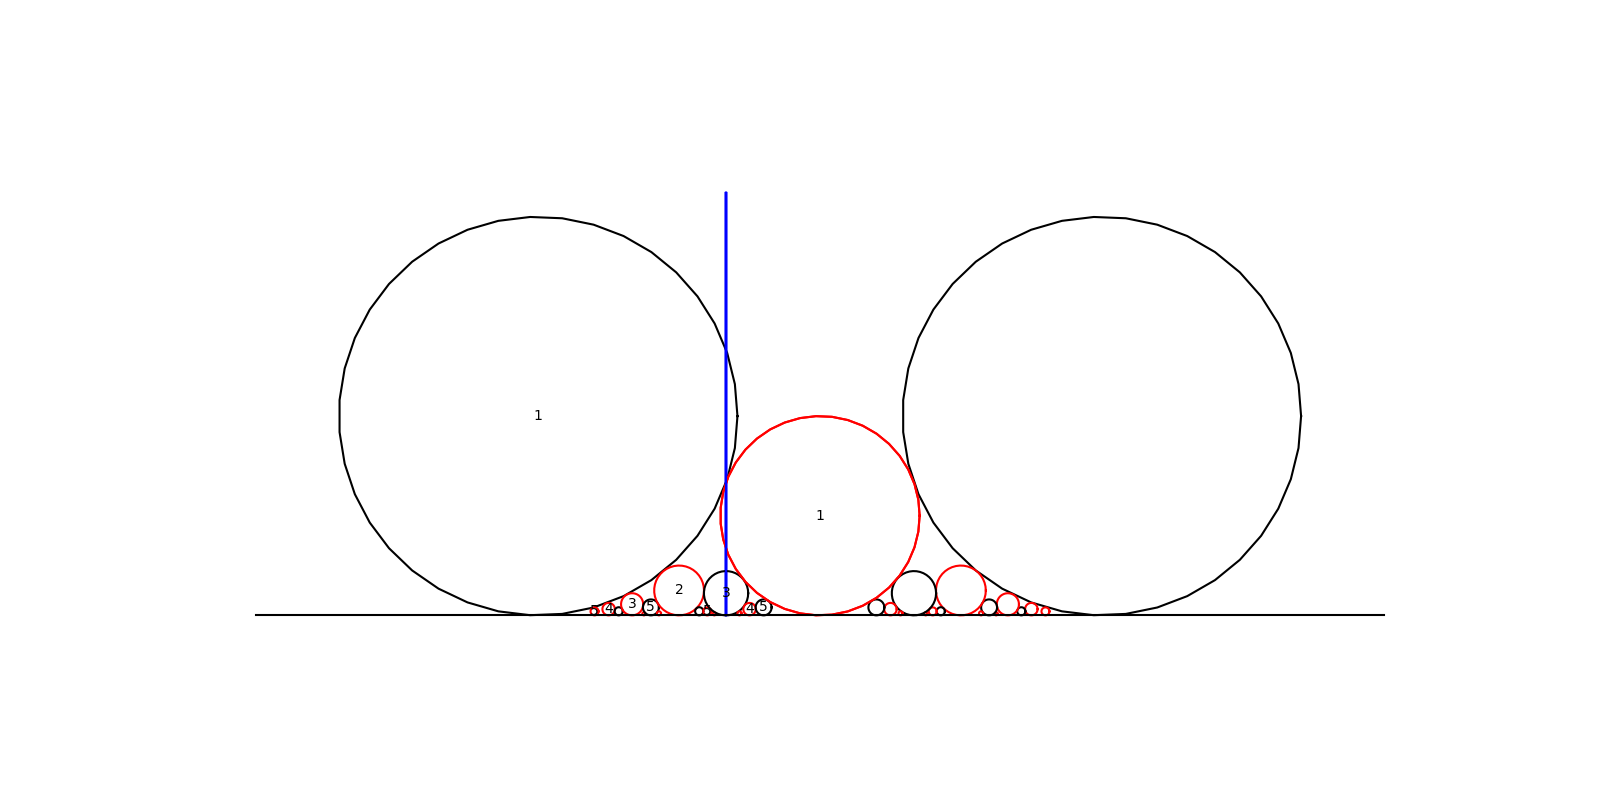
\includegraphics[scale=1]{farey_mod.png} 
\end{center}
\caption{Modified Farey circles}
\label{modified farey}
\end{figure}

\subsection{Arcs on $\oot$}

The surface has two cusps and so there are two kind of arc
\begin{itemize}
	\item arcs that join distinct cusps $0/1$ and $1/0$
	\item arcs that have both ends at the same either
		cusps $0/1$ or $1/0$.
\end{itemize}

\begin{lem}
Arcs of the first kind,
that is those which join distinct cusps $0/1$ and $1/0$,
have the same $\lambda$-length for the inherited
cusp regions and our modified cusp regions. 
\end{lem}


Since the automorphism swaps cusps only arcs of the first  kind can be invariant for it.
Now any arc of the first kind lifts to a vertical line ending at
some rational $\frac{m}{n}\in \QQ$.
It follows that for each  $p$  prime there are exactly $p-1$ arcs of the first kind,
namely the projections to $\oot$ of the Poincaré geodesics  $\infty,
\frac{2k}{p}$ with  $k = 1,2\ldots p-1$
and each of these has $\lambda$-length $p$ for our choice of cusp regions.


\thebibliography{99}

\bibitem{aigner}
M. Aigner
\textit{Markov's Theorem and 100 Years of the Uniqueness Conjecture}, Springer( 2013)


\bibitem{aigner2}
Aigner M., Ziegler G.M.  
\textit{Representing numbers as sums of two squares.} In: Proofs from the book. Springer, Berlin, Heidelberg. (2010)

\bibitem{barag}
A. Baragar,
\textit{On the Unicity Conjecture for Markoff Numbers}
Canadian Mathematical Bulletin , Volume 39 , Issue 1 , 01 March 1996 , pp. 3 - 9

\bibitem{button}
J. O. Button, 
\textit{The uniqueness of the prime Markoff numbers},
 J. London Math. Soc.
(2) 58 (1998), 9–17.

\bibitem{frieze}
Ilke Canakci, Anna Felikson, Ana Garcia Elsener, Pavel Tumarkin,
\textit{Friezes for a pair of pants}a,
Proceedings of the Formal Power Series and Algebraic Combinatorics 2022 - Séminaire Lotharingien de Combinatoire
% \bibitem{cana}
% Ilke Canakci, Ralf Schiffler
% \textit{Snake graphs and continued fractions}
% European Journal of Combinatorics
% Volume 86, May 2020, 103081

\bibitem{dolan}
Dolan, S., A very simple proof of the two-squares theorem. The Mathematical Gazette, 105(564), 511-511. (2021) doi:10.1017/mag.2021.120

\bibitem{elsholtz}
Elsholtz C.A 
\textit{Combinatorial Approach to Sums of Two Squares and Related Problems.}
 In: Chudnovsky D., Chudnovsky G. (eds) Additive Number Theory. Springer, New York, NY.
 (2010) 

\bibitem{Fomin}
S. Fomin and D. Thurston,
\textit{Cluster algebras and triangulated surfaces}
Part II: Lambda lengths, \url{arXiv:1210.5569v1.}

\bibitem{ford}
Lester R Ford,
\textit{Automorphic Functions}

\bibitem{generalov}
Generalov, A.I. A combinatorial proof of Euler-Fermat’s theorem on the representation of the primes p=8k+3 by the quadratic form $x^2 + 2y^2$. J Math Sci 140, 690–691 (2007). https://doi.org/10.1007/s10958-007-0008-6

\bibitem{heath}
Heath-Brown, Roger. 
\textit{ Fermat’s two squares theorem.} Invariant (1984) 

\bibitem{herriot}
Neil Herriot, Communication with Jim Propp
\url{https://faculty.uml.edu/jpropp/reach/Herriot/ptolemywriteup.html}

\bibitem{jackson}
Jackson, Terence H.. “A Short Proof That Every Prime $p = 3 (\mod 8)$
Is of the Form $x^2 + 2y^2$.” The American Mathematical Monthly 107 (2000): 447 - 447.


\bibitem{mong}
M.L. Lang, S.P Tan,
\textit{A simple proof of the Markoff conjecture for prime powers}
Geometriae Dedicata volume 129, pages15–22 (2007)


\bibitem{thesis}
G. McShane,
\textit{Simple geodesics and a series constant over Teichmuller space}
Invent. Math. (1998)


\bibitem{north}
Northshield, Sam. 
\textit{A Short Proof of Fermat’s Two-square Theorem.} The American Mathematical Monthly. 127. 638-638. (2020). 


\bibitem{bob}
R. C. Penner, 
\textit{The decorated Teichmueller space of punctured surfaces}, 
Communications in Mathematical Physics 113 (1987), 299–339.

% \bibitem{propp}
% James Propp,
% The combinatorics of frieze patterns and Markoff numbers,
% \url{https://arxiv.org/abs/math/0511633}

\bibitem{propp}
James Propp,
The combinatorics of frieze patterns and Markoff numbers,
in  Integers, Volume 20 (2020)
\url{http://math.colgate.edu/~integers/u12/u12.pdf}


\bibitem{serre}
J-P. Serre,
\textit{A Course in Arithmetic},
Graduate Texts in Mathematics,
Springer-Verlag New York
1973

\bibitem{springborn1}

B. Springborn. The hyperbolic geometry of Markov’s theorem on Diophantine
approximation and quadratic forms. Enseign. Math., 63(3-4):333–373, 2017.

\bibitem{springborn2}
Boris Springborn,
\textit{The worst approximable rational numbers}
\url{https://arxiv.org/abs/2209.15542}



% \bibitem{saw}
% Scott Wolpert,
% \textit{On the Kahler form of the moduli space of once-punctured tori}, 
% Comment. Math. Helv. 58(1983)246-256

\bibitem{zagier}
D. Zagier,
 \textit{A one-sentence proof that every prime p = 1 (mod 4) is a sum of two squares}, 
 American Mathematical Monthly, 97 (2): 144
 
 % \bibitem{zhang}
 % Y. Zhang,
 % \textit{ An elementary proof of uniqueness of Markoff numbers}
 % preprint, arXiv:math.NT/0606283
 
  % \bibitem{zhang2}
  %  Y. Zhang,
 % \textit{Congruence and uniqueness of certain Markoff numbers}
 % Acta Arithmetica, Volume: 128, Issue: 3, page 295-301

\end{document}
